\subsection{Loi exponentielle - minimisation aléatoire}
Cette méthode a pour but de générer des nombres pseudos aléatoires selon une loi exponentielle de la forme :
\begin{equation}
f(x) = 
\left\lbrace
	\begin{array}{ccc}
   	 1 - e^{-\lambda x} & \text{si x $\geq$ 0}\\ 
   	 0 & \text{sinon}
    \end{array}\right.
\end{equation}
\smallbreak
Nous avons déjà vu une méthode permettant de faire ça, mais nous devions calculer un logarithme, ce que nous voulons éviter. C'est pour cela que nous avons mis cette méthode en place.\\ \smallbreak
Soit $Q[k] = \frac{ln 2}{1!} + \frac{(ln 2)^2}{2!} + \frac{(ln 2)^3}{3!} + ... + \frac{(ln 2)^k}{k!}$\\ \smallbreak
On voit que $ Q[k] \rightarrow 1$ quand $k \rightarrow +\infty$. En effet, Q[k] représente le développement de Taylor sans le premier terme ($ + 1$) de $e^{ln(2)} = 2$. On a donc que ça tend vers $2 - 1 = 1$.\\ \smallbreak
En pratique on s'arrête quand $Q[k] > 1 -2^{1-n}$ pour des mots de n bits.\\ \smallbreak
\begin{algorithm}[H]
	\caption{Algorithme minimisation aléatoire}
	\begin{algorithmic}[1]
		\State Générer un nombre aléatoire suivant la loi uniforme $V = (b_{0}, b_{1}, ..., b_{n})$ (en binaire). Soit j le premier bit étant 1 ($P\{j = J\} = \frac{1}{2^{J+1}}$). Alors, soit $U = (b_{j+1},...,b_{n})$.\smallbreak
		\State Si $U < ln(2)$, alors $X \leftarrow \mu (j\,ln(2) + U)$ et on arrête l'algorithme ici.\smallbreak
		\State Trouver la plus petite valeur de k telle que $Q[k] > U$, générer k nombres aléatoires $U_{1}, U_{2}, ..., U_{k}$ . $V \leftarrow min(U_{1}, U_{2}, ..., U_{k})$\smallbreak
		\State Prendre $X \leftarrow \mu (j + V)\,ln(2)$
	\end{algorithmic}
\end{algorithm} 

L'algorithme est très facile à appliquer. Il faut juste comprendre pourquoi on obtient bien un nombre suivant une loi exponentielle.\\
Calculons la fonction de répartition de X et regardons si nous obtenons bien la fonction de répartition de la loi exponentielle ($1 - e^{-\lambda x}$).\\
\begin{equation}
\begin{split}
	P\{X \leq X_0\} =& (ln(2))\,P\left\{\mu(j\,ln(2) + U) \leq X_0\right\} +\\
	& \sum_{k=2}^{+\infty}\frac{(ln(2))^k}{k!}\,P\left\{\mu(j + V)\,ln(2) \leq X_0\right\}
\end{split}
\end{equation}
\smallbreak
La première ligne provient de la 2\ieme ligne de l'algorithme et la seconde provient de la $4^{eme}$ ligne de l'algorithme.
\paragraph{1ère ligne du calcul}
\begin{itemize}
\item ln(2) s'explique car on a $U<ln(2)$ (probabilité qu'un truc uniforme < X = X)
\item Le reste exprime juste $P\{X \leq X_0\}$ dans le cas où on est dans la seconde ligne de l'algo.
\end{itemize}
\paragraph{2ème ligne du calcul}
\begin{itemize}
\item La somme exprime les $U<Q[k]$ par le même raisonnement qu'au-dessus (probabilité qu'un truc uniforme < X = X), et vu qu'on a plusieurs k tq $U<Q[k]$, on obtient une somme sur les Q[k]. On commence cette somme à 2 puisque le cas $k=1$ est impossible puisque $U > ln(2)$ dans ce cas-ci.
\item Encore une fois, le reste exprime juste $P\{X \leq X_0\}$ dans le cas où on est dans la quatrième ligne de l'algo.
\end{itemize}
\smallbreak
Suite du calcul : \\ 
\begin{equation}
\begin{split}
=& (ln(2))\,P\left\{j + \frac{U}{ln(2)} \leq \frac{X_0}{\mu\,ln(2)}\right\} +\\
	& \sum_{k=2}^{+\infty}\frac{(ln(2))^k}{k!}\,P\left\{(j + V) \leq \frac{X_0}{\mu\,ln(2)}\right\}
\end{split}
\end{equation}

\begin{figure}[H]
    \includegraphics[width=\textwidth]{Dorian1}
\end{figure}
\begin{figure}[H]
    \includegraphics[width=\textwidth]{Dorian2}
\end{figure}
\begin{figure}[H]
    \includegraphics[width=\textwidth]{Dorian3}
\end{figure}
\begin{figure}[H]
    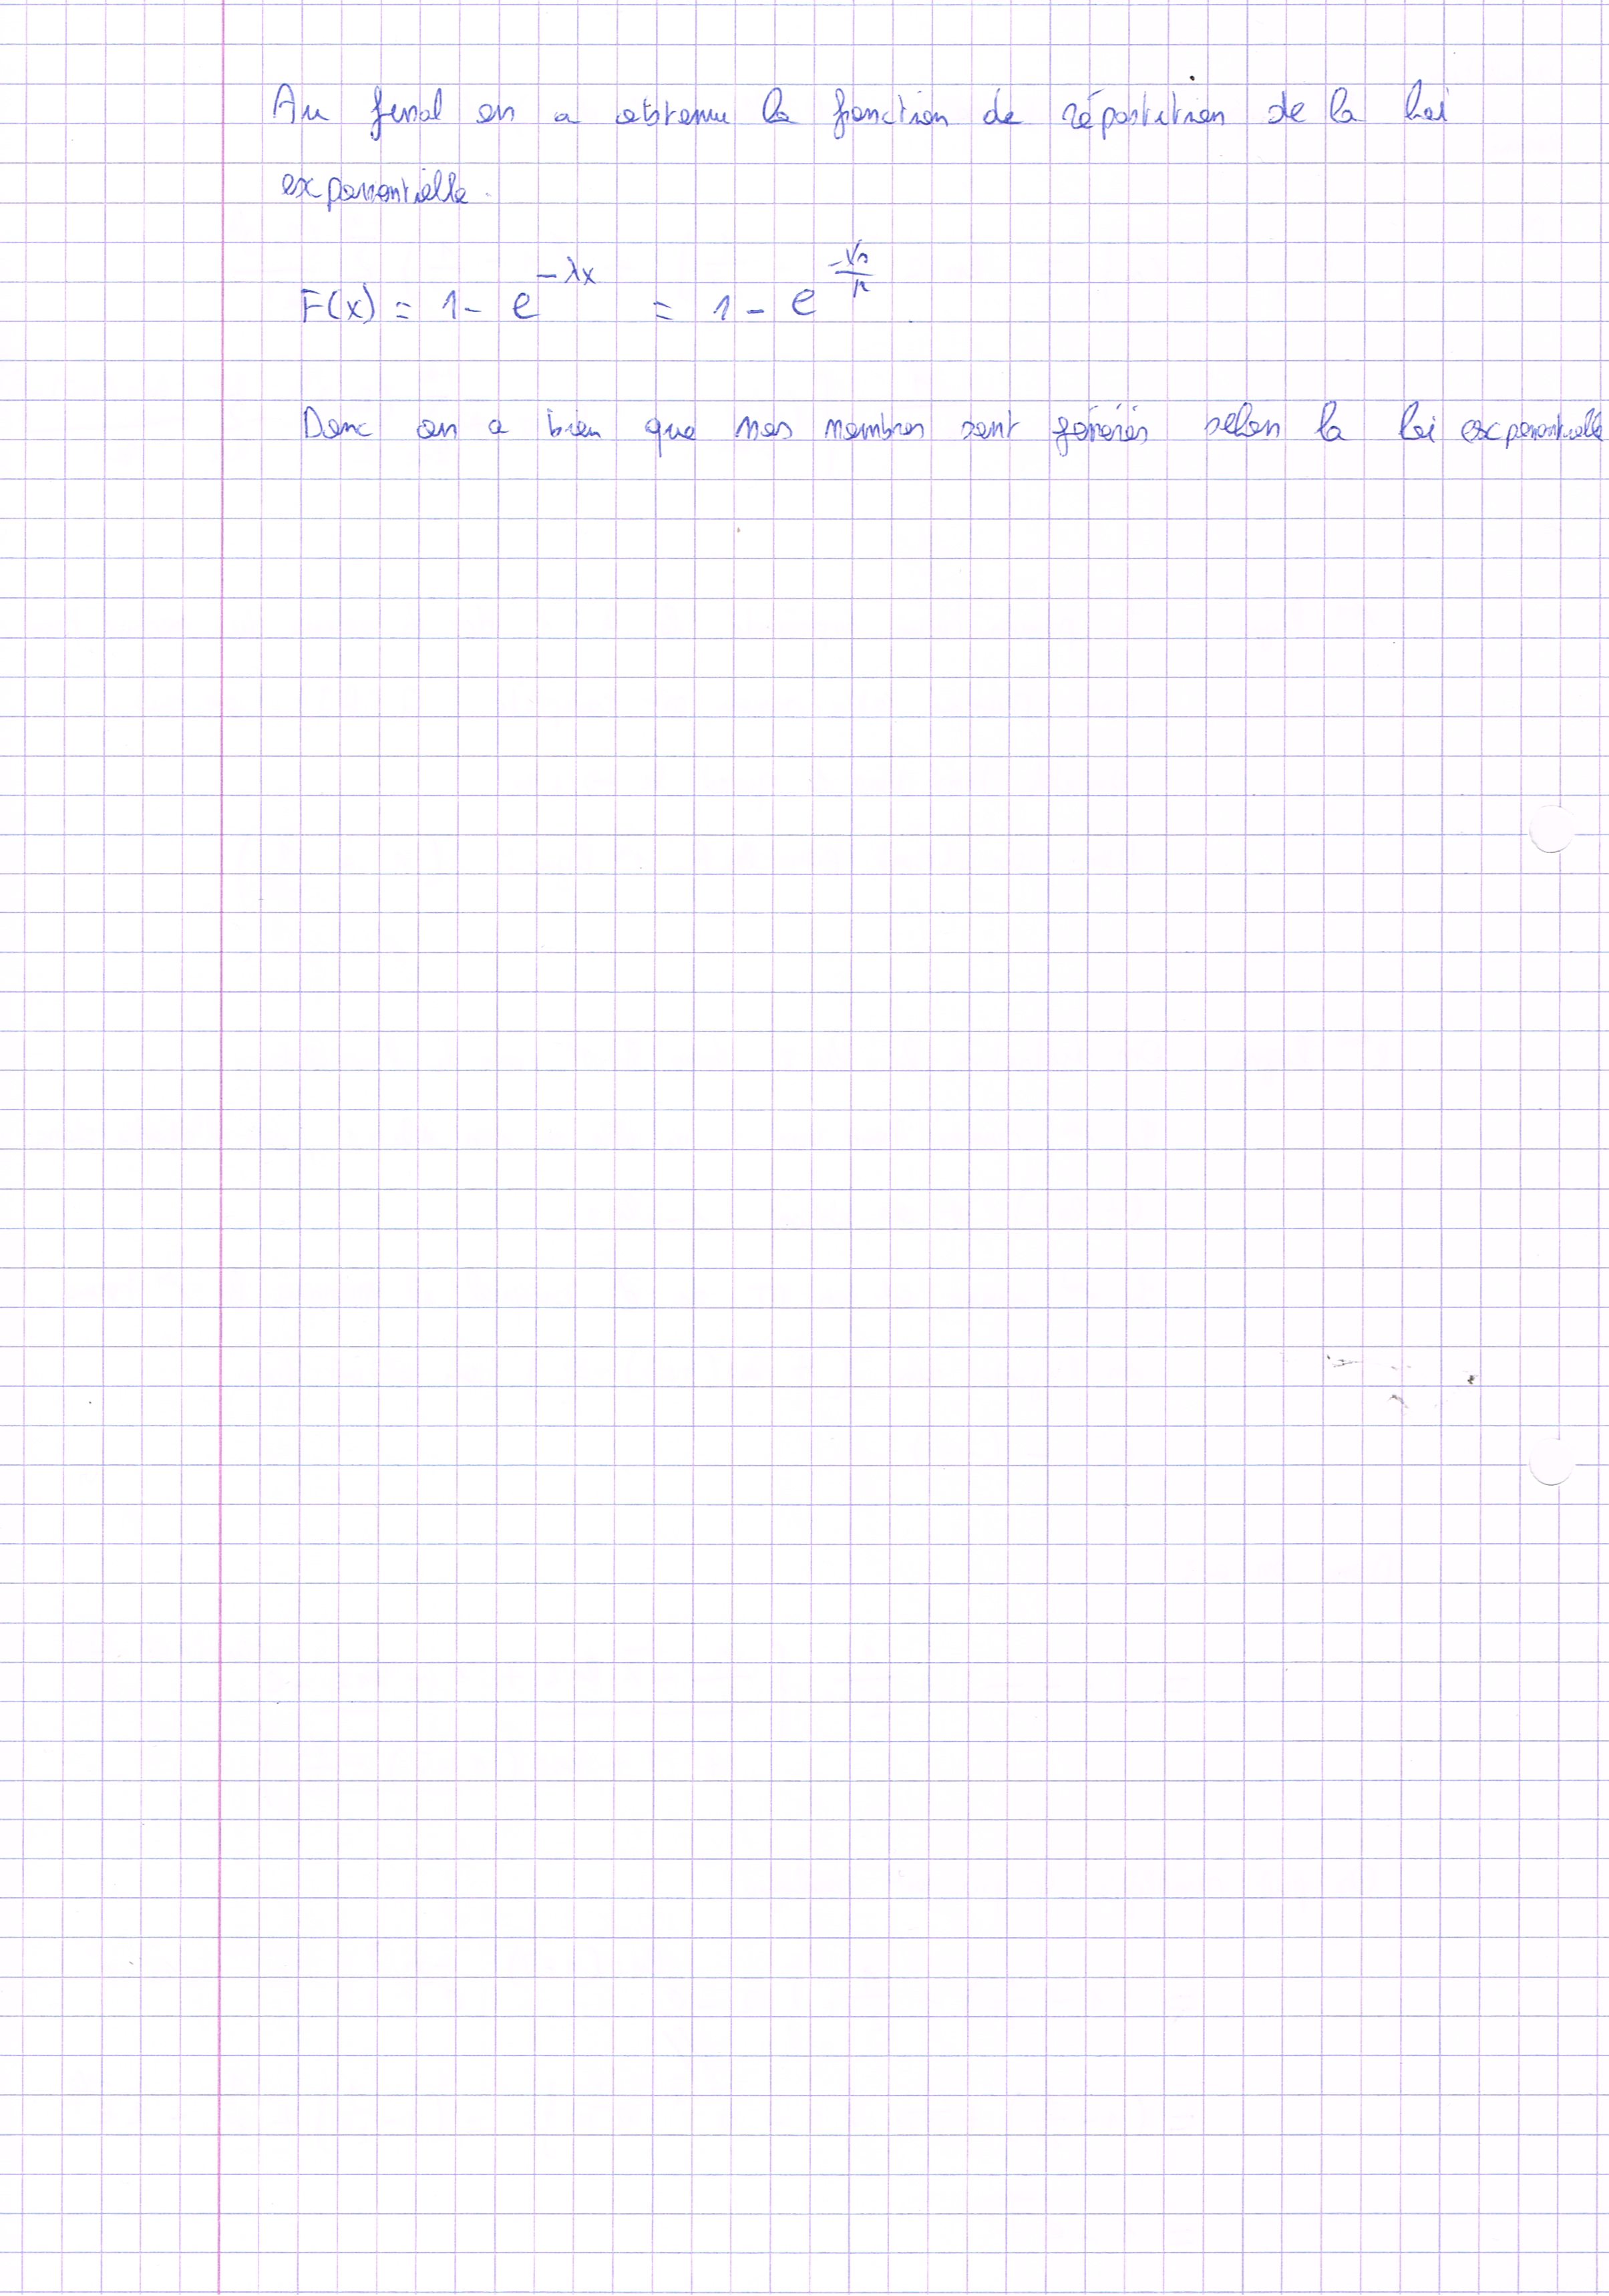
\includegraphics[width=\textwidth]{Dorian4}
\end{figure}